\documentclass[ngerman,landscape,twocolumn]{adtexsheet}

 %for pseudocode
 %http://tug.ctan.org/macros/latex/contrib/algorithm2e/doc/algorithm2e.pdf
\usepackage[ruled,noend,noline,nofillcomment,linesnumbered,]{algorithm2e}
\DontPrintSemicolon
\SetKwFor{For}{for }{}{}
\SetKwFor{While}{while }{}{}
\SetKwIF{If}{ElseIf}{Else}{if}{}{else if}{else}{}
\SetKw{Return}{return}
\newcommand{\To}{\KwTo}
\newcommand{\swap}{\leftrightarrow}
\newcommand*{\CommentInLine}{\tcc*[f]}
\newcommand{\todo}{\colorbox{red}{\textbf{Muss noch was gemacht werden}}}
\usepackage{mathtools}
\usepackage{tabularx}
\DeclarePairedDelimiter\ceil{\lceil}{\rceil}
\DeclarePairedDelimiter\floor{\lfloor}{\rfloor}
\DeclarePairedDelimiter\abs{|}{|}

\usepackage[T1]{fontenc}

\exnumber{6}
%Teilnehmer
%<Name> & <Gruppennummer> & <Kreuz Aufgabe 1> & <Kreuz Aufgabe 2> & <Kreuz Aufgabe 3> & <Kreuz Aufgabe 4>
\participantOne{Theodor Bajusz&5&x&x&x&x&x}
\participantTwo{Valerij Dobler&13&x&x&x&x&x}
\participantThree{Matz Radloff&6&x&x&x&x&x}
\participantFour{Robin Wannags&5&x&x&x&x&x}

% sheet specific notions and notation,
%drawing automatons
\usepackage{tikz}
\usepackage{listings}
\usepackage{xcolor}
\usetikzlibrary{shapes}
\usepackage{listings}
\usepackage{stmaryrd}

\begin{document}

\begin{question}
    \begin{figure}
        \centering
        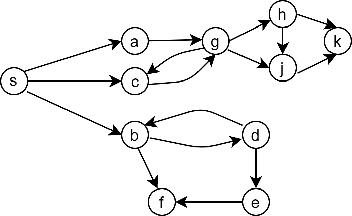
\includegraphics[width=.5\linewidth]{images/ex6q1.png}
        \label{fig:my_label}
    \end{figure}
    \begin{enumerate}
        \item Führen Sie die Tiefensuche ausgehend von dem Knoten s aus. Falls es mehrere Möglichkeiten gibt einen Knoten auf den Stack zu pushen, entscheiden Sie sich für den Knoten mit der kleinsten lexikographischen Ordnung (alphabetische Ordnung). Zeichnen Sie den Graphen, der hierbei entsteht, mit den jeweiligen Zeitstempeln. (2 Punkte)
        
       
        \item Führen Sie die Breitensuche ausgehend von dem Knoten s aus. Falls es mehrere Möglichkeiten gibt einen Knoten auf den Queue hinzuzufügen, entscheiden Sie sich für den Knoten mit der kleinsten lexikographischen Ordnung (alphabetische Ordnung). Zeichnen Sie den Graphen, der hierbei entsteht, mit den jeweiligen Distanzen. (1 Punkte)
        
    \end{enumerate}
\end{question}

\begin{solution}
    \begin{enumerate}
        \item In Abbildung \ref{fig:DFS-Tree} steht die erste Zahl für den Zeitpunkt der Entdeckung und die zweite Zahl für den Zeitpunkt der vollständigen Abarbeitung.
        \item In Abbildung \ref{fig:BFS-Tree} steht die Zahl für den Abstand zum Startknoten.
    \end{enumerate}
        \begin{figure}
            \hfill
            \newcommand{\sep}{0.23}
            \tikzstyle{every node}=[circle,draw=black]
            \minipage[t]{\sep\textwidth}
                \centering
            \tikzstyle{every node}=[circle,draw=black]
        \begin{tikzpicture}[->,sibling distance=20mm,level distance=20mm]
            \node{s,1-22} 
                child { node{a,2-13}
                    child { node{g,3-12}
                        child { node{c,4-5} }
                        child { node{h,6-11}
                            child { node{j,7-10}
                                child { node{k,8-9}}
                            }
                        }
                    }
                }
                child { node{b,14-21}
                    child[missing] {}
                    child { node{d,15-20}
                        child { node{e,16-19}
                            child { node{f,17-18}}
                        }
                    }
                }
                ;
                \end{tikzpicture}
                \centering
                \caption{Tiefensuchbaum zu 1a)}
                \label{fig:DFS-Tree}
            \endminipage\hfill
            \minipage[t]{\sep\textwidth}
        \begin{tikzpicture}[->,sibling distance=20mm,level distance=20mm]
            \node{s,0} 
                child { node{a,1}
                    child { node{g,2}
                        child { node{h,3}
                            child { node{k,4}}
                        }
                        child { node{j,3}}
                    }
                }
                child { node{b,1}
                    child[missing]{}
                    child { node{d,2}
                        child { node{e,3}}
                    }
                    child {node {f,2}}
                }
                child { node{c,1}}
                ;
                \end{tikzpicture}
                \centering
                \caption{Breitensuchbaum zu 1b)}
                \label{fig:BFS-Tree}
            \endminipage
        \end{figure}
\end{solution}

\newpage

% Aufgabe 2
\begin{question}
    \begin{enumerate}
        \item Beschreiben Sie wie das folgende Problem als Graph modelliert werden kann. Sie befinden sich in einem quadratischen Gitter mit der Kantenlänge $m$. Sie starten an der Position $(1, 1)$ und möchten zur Position $(m, m)$ gelangen. Der Output ist die Anzahl an Schritten, die man benötigt, um zur Position $(m, m)$ zu gelangen. In einem Schritt können Sie sich vertikal oder horizontal von einem freien Platz zu einem anderen freien Platz bewegen. Unten finden Sie ein Beispiel mit $m = 4$ (1 Punkte)
        
        \item Nehmen Sie an, dass man die Anzahl der Schritte minimieren möchte. Beschreiben Sie einen Algorithmus, der berechnet wie viele Schritte man braucht um von $(1,1)$ zur Position $(m, m)$ in $O(m^2)$ zu gelangen. Begründen Sie \textbf{kurz} die Korrektheit des Algorithmus', sowie die Einhaltung der asymptotischen Laufzeitschranke. \textbf{Hinweis}: Es kann auch sein, dass es keine Lösung gibt! In diesem Fall geben sollte der Algorithmus $\infty$ zurückgeben. (2 Punkte)
    \end{enumerate}
\end{question}

\begin{solution}
    \begin{enumerate}
        \item  Wir können das Problem als Graph modellieren indem wir jede freie Zelle als Knoten mit maximal $4$ Nachbarn in unsere Knotenmenge aufnehmen.

        Wir kodieren jeden Knoten $V=(x,y)$, wobei $1 \leq x \leq m$ und $1 \leq y \leq m$ die Koordinaten im Gitter sind. Wenn die direkten Nachbarn $\{(x-1,y-1),(x+1,y-1),(x-1,y+1),(x+1,y+1) \}$ vom Knoten $V$ nicht mit "X" markiert sind und sich innerhalb des Gitters befinden, werden die Nachbarn zu $V$ mit einer Kante verbunden, Duplikate werden dabei ignoriert. Dabei entsteht ein ungerichteter Graph.

        Nun müssen wir nur noch eine Breitensuche auf dieser Knotenmenge durchführen und haben damit einen gültigen Weg um von $(1,1)$ zu $(m,m)$ zu gelangen, falls diese Zelle erreichbar ist.
        
        \item Wir führen eine Breitensuche (\textsc{BFS}), so wie sie in der Vorlesung eingeführt wurde, von $(1,1)$ aus in dem in Aufgabe 2a) beschriebenen Graphen aus. Für die Laufzeit von \textsc{BFS} ergibt sich 
        $$O(|V|+|E|) \leq O(|V|+|V|^2) \leq O(2|V|^2) = O(m^2).$$
        Da die \textsc{BFS} bei uniformen Kantengewichten, ein \textsc{Single-Source Shortest Path}-Algorithmus ist, bekommen wir als Ergebnis auch den kürzesten Weg von $(1,1)$ nach $(m,m)$, hier auch nur wenn dieser existiert, also die Zielzelle erreichbar ist. Die Länge des kürzesten Pfads ist dann die Anzahl der Schritte, welche minimal benutzt werden müssen um vom Start- zum Zielpunkt gelangen zu können.
        
        Wenn die Zielzelle nicht erreichbar ist, ist der Weg dorthin $\infty$ Schritte weit. Und die Korrektheit folgt aus der Korrektheit des \textsc{BFS}. \hfill \qedsymbol
        
    \end{enumerate}
\end{solution}

% Aufgabe 3
\begin{question}
Sei $G = (V, E)$ ein Graph. Nehmen Sie für die folgende Aufgabe an, dass Sie den Input $G$ als Adjazenzliste kodiert erhalten. Geben Sie einen Algorithmus in Pseudocode an, der in $O(|V | + |E|)$ die Anzahl der Zusammenhangskomponenten berechnet. Begründen Sie kurz die Korrektheit des Algorithmus', sowie die Einhaltung der asymptotischen Laufzeitschranke. (3 Punkte)
\end{question}

\definecolor{codegreen}{rgb}{0.4,0.4,0.4}
\definecolor{codegray}{rgb}{0.7,0.7,0.7}
\definecolor{codepurple}{rgb}{0.2,0.3,0.9}
\definecolor{backcolor}{rgb}{0.9,0.9,0.9}

    \begin{lstlisting}[
    basicstyle=\small,
    language=Java,
    numbers=left,                    
    numbersep=0pt,
    backgroundcolor=\color{backcolor},
    commentstyle=\color{codegreen},
    keywordstyle=\color{codepurple},
    numberstyle=\tiny\color{codegray},
    stringstyle=\color{codepurple},
    basicstyle=\ttfamily\footnotesize,
]
public Long getConnectedComponentCount(
        Map<Long, Set<Long>> adjazenzMap) {
    Long componentCount = 0L;
    Queue<Long> queue = new LinkedList<>();
    
    // iteriere solange, bis die adjazenzMap leer ist
    while (!adjazenzMap.isEmpty()) {
      
      // hol einen beliebigen Entry aus der Map und queue ihn
      queue.offer(adjazenzMap.entrySet().iterator().next().getKey());
      List<Long> componentList = new ArrayList<>();
      
      // arbeite die Queue ab
      while (!queue.isEmpty()) {
        Long head = queue.poll();
        
        // fuege den key zur Komponentenliste, falls nicht vorhanden
        if (!componentList.contains(head)) {
          componentList.add(head);
        }
        // fuege die values zur Komponentenliste und queue sie, 
        // falls nicht vorhanden
        for (var value : adjazenzMap.get(head)) {
          if (!componentList.contains(value)) {
            componentList.add(value);
            queue.offer(value);
          }
        }
        // remove key+value aus der Map wenn diese abgearbeitet wurden
        adjazenzMap.remove(head);
      }
      // wenn die Queue leer ist -> Komponente gefunden
      componentCount++;
    }
    return componentCount;
  }
\end{lstlisting}
Der Algorithmus funktioniert für ungerichtete Graphen, da in der Aufgabenstellung nicht explizit erwähnt wurde für welche Art von Graphen wir ihn entwickeln sollten. Da es sich jedoch um Zusammenhangskomponenten handelt, und nicht um strenge oder schwache Zusammenhangskomponenten, sind wir davon ausgegangen dass es sich um einen ungerichteten Graphen handeln muss.

In diesem Code nutzen wir eine Map, anstelle von einer LinkedList, als Adjazenzliste. Dies ändert jedoch nichts an der Funktionsweise des Algorithmus. Der Key gibt das Element an, um welches es sich handelt und das Set alle direkten Nachbarn, äquivalent zu der Adjazenzliste aus der Vorlesung.

\emph{Laufzeit:} Die beiden while Schleifen haben zusammen eine Laufzeit von $|V|$. Dies wird ersichtlich, wenn man sich die Funktion der beiden Schleifen ansieht, denn die erste while-Schleife (Zeile 7) wird erst verlassen, wenn die AdjazenzMap leer ist, jedoch werden die Elemente der Map in der zweiten while-Schleife entfernt (Zeile 14). Jedes Element muss also entfernt werden und wird genau einmal entfernt, somit wird die innere while-Schleife genau V mal betreten, die äußere hat hierauf keinen Einfluss. Die for-Schleife (Zeile 23) wird für jeden Nachbarn in der Map genau einmal betreten. Hierbei können Nachbarn doppelt zählen, wenn sie ein Nachbar von mehreren Knoten sind. Diese Schleife wird also genau $|E|$ mal betreten und zwar unabhängig von den while-Schleifen.

Die restlichen Zeilen sind von linearer Zeit und können vernachlässigt werden, weshalb sich insgesamt eine Laufzeit von $O=(|V|+|E|)$ ergibt.

% Aufgabe 4
\begin{question}
    Beweisen Sie die folgenden Behauptungen über Graphen und minimale Spannbäume:
    \begin{enumerate}
        \item Sei $G = (V, E)$ ein Graph und $e \in E$ eine Kante, die auf keinem Kreis liegt. Dann ist $e$ in jedem minimalen Spannbaum enthalten. (2 Punkte)
        \item Sei $G$ ein ungerichteter, zusammenhängender Graph mit paarweise verschiedenen Kantengewichten. Dann existiert nur ein einziger minimaler Spannbaum von $G$, d.h. der minimale Spannbaum ist eindeutig. (3 Punkte)
    \end{enumerate}
\end{question}

\begin{solution}
    \begin{enumerate}
       \item 
       Sei eine Kante $f \in E$ , die auf keinem Kreis liegt und nicht in jedem minimalen Spannbaum enthalten ist. Um den minimalen Spannbaum zu bilden, müssen beide Knoten durch Pfade erreicht werden, welche $f$ nicht enthalten. Wenn allerdings mehrere Pfade zwei Knoten verbinden, handelt es sich um einen Kreis und die Kante $f$ muss in diesem Kreis liegen. Dies widerspricht der Annahme und $f$ muss in jedem minimalen Spannbaum enthalten sein.
       \item
       Wir nehmen an es gäbe zwei verschiedene Minimale Spannbäume $A$ und $B$ des Graphen $G$, wobei gilt dass die Menge der Kanten aus $G$ paarweise verschieden sind. Da $A$ und $B$ unterschiedlich sind gibt es mindestens eine Kante die zu einem der Spannbäume gehört, jedoch nicht zu dem anderen. Von diesen Kanten sei $e_1$ die Kante mit dem geringsten Gewicht. O.b.d.A. nehmen wir an, dass $e_1 \in A$. Durch $B \cup e_1$ entsteht ein Zyklus $C$. Da $A$ ein Baum ist, enthält dieser keinen Zyklus, daher muss es in $C$ eine Kante $e_2$ geben, welche nicht in $A$ ist. Da $A$ ein minimaler Spannbaum ist und $e_1$ die Kante mit dem geringsten Gewicht ist, muss $e_2$ $>$ $e_1$ gelten. Wenn wir nun $e_2$ mit $e_1$ in $B$ ersetzen, würden wir einen "minimaleren" \,Spannbaum erhalten was gegen die Annahme spricht, dass $B$ bereits minimal sei.
    \end{enumerate}
\end{solution}

% Aufgabe 5
\begin{question}
    \begin{figure}
        \centering
        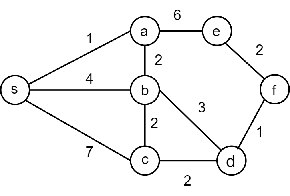
\includegraphics[width=.4\linewidth]{images/ex6q5.png}
        \label{fig:my_label}
    \end{figure}
    \begin{enumerate}
        \item Wenden Sie Dijkstras Algorithmus auf den oben dargestellten Graphen an. Geben Sie tabellarisch die am Ende jeder Iteration der While-Schleife in der Queue enthaltenen Keys an. (2 Punkte)
        \item Modifizieren Sie den Pseudocode von Dijkstras Algorithmus so, dass er als Input einen Graphen, einen Startknoten $s$ und einen Zielknoten $v$ als Input nimmt und als Output die explizite Darstellung des kürzesten Pfades von $s$ nach $v$ als Sequenz von Knoten ausgibt. Begründen Sie \textbf{kurz} die Korrektheit Ihrer Lösung. (3 Punkte)
    \end{enumerate}
\end{question}

\begin{solution}
    
\begin{enumerate}
    \item
    \begin{tabular}[h]{c|c|c|c|c|c|c|c|c}
        \hline
        Iteration & & s & a & b & c & d & e & f\\
        \hline
            0 (Initialisierung)& Gewichtung & 0 & $\infty$ & $\infty$ & $\infty$ & $\infty$ & $\infty$ & $\infty$ \\
              & Vorgänger & $\diagup$ & $\diagup$ & $\diagup$ & $\diagup$ & $\diagup$ & $\diagup$ & $\diagup$\\   
        \hline
            1(s)& Gewichtung  & 0 & 1 & 4 & 7 & $\infty$ & $\infty$ & $\infty$\\
              & Vorgänger &$\diagup$ & s & s & s & $\diagup$ & $\diagup$ & $\diagup$ \\   
        \hline
            2(a)& Gewichtung  & 0 & 1 & 3 & 7 & $\infty$ & 7 & $\infty$\\
              & Vorgänger &$\diagup$ & s & a & s & $\diagup$ & a & $\diagup$ \\  
        \hline
            3(b)& Gewichtung  & 0 & 1 & 3 & 5 & 6 & 7 & $\infty$\\
              & Vorgänger &$\diagup$ & s & a & b & b & a & $\diagup$\\
        \hline
            4(c)& Gewichtung  & 0 & 1 & 3 & 5 & 6 & 7 & $\infty$\\
              & Vorgänger &$\diagup$ & s & a & b & b & a & $\diagup$\\
        \hline
            5(d)& Gewichtung  & 0 & 1 & 3 & 5 & 6 & 7 & 7\\
              & Vorgänger &$\diagup$ & s & a & b & b & a & d\\
        \hline
            6(e)& Gewichtung  & 0 & 1 & 3 & 5 & 6 & 7 & 7\\
              & Vorgänger &$\diagup$ & s & a & b & b & a & d\\
        \hline
            7(f)& Gewichtung  & 0 & 1 & 3 & 5 & 6 & 7 & 7\\
              & Vorgänger &$\diagup$ & s & a & b & b & a & d\\
    \end{tabular}
    \item Um den kürzesten Pfad auszugeben müssen wir den Dijkstra-Algorithmus wie folgt erweitern:
    
        Nach der While-Schleife sind die Vorgänger für den kürzesten Pfad in allen Knoten gespeichert. Durch den Aufruf $\pi (w)$ können wir somit den Vorgängerknoten eines Knoten $w \in V$ bekommen. Nun können wir mit unserem gewünschten Zielknoten $v$ den Vorgängerknoten $v'$ herausfinden, von dem wir mit $\pi (v')$ widerrum den Vorgänger rekursiv bestimmen können. Dies müssen wir solange durchführen, bis wir als Vorgänger-knoten unseren gewählten Startknoten $s$ bekommen. Wir können die Folge nun als Lösung ausgeben lassen.
        
        Da im Algorithmus immer der Vorgänger des kürzesten Pfades gespeichert wird können wir hierdurch schnell den gesamten kürzesten Pfad finden, indem wir ihn rückwärts durchlaufen. Da ausschließlich der Vorgänger des kürzesten Pfades gespeichert wird, kann logischerweise auch nur dieser durchlaufen werden, womit die Korrektheit begründet ist.
       
\end{enumerate}
\end{solution}
     
 \begin{lstlisting}[
    basicstyle=\small,
    language=Java,
    numbers=left,                    
    numbersep=0pt,
    backgroundcolor=\color{backcolor},   
    commentstyle=\color{codegreen},
    keywordstyle=\color{codepurple},
    numberstyle=\tiny\color{codegray},
    stringstyle=\color{codepurple},
    basicstyle=\ttfamily\footnotesize,
    mathescape=true,
]
Dijkstra2(G, w, s, v)
    for u $\in$ V
        key(u) $\gets \infty$
        $\pi$(u) $\leftarrow$ NIL

    key(s) $\leftarrow$ 0
    Q $\leftarrow$ BuildHeap(V)
    while Q $\neq$ $\emptyset$
        u $\leftarrow$ DeleteMin(Q)
        for x $\in$ Adj(u)
            if key(x) > key(u) + w(u, x)
                DecreaseKey(Q, x, key(u) + w(u, x))
                $\pi$(x) $\leftarrow$ u
    
    out $\leftarrow$ Array
    i $\leftarrow$ $\pi$(v)
    out[0] $\leftarrow$ v
    while i != s
        out.append(i)
        i = $\pi$(i)
        
    return reversed(out)

\end{lstlisting}
% Aufgabe 6
\begin{question}
    Erarbeiten Sie sich anhand der Fachliteratur das Konzept der topologischen Sortierung von Graphen (z.B. in [Introduction to Algorithms, 3rd edition] Seite 612ff) und bearbeiten Sie die folgenden Aufgaben: 
    \begin{enumerate}
        \item Im Allgemeinen wird die topologische Sortierung für sogenannte DAGs (directed acyclic graphs) definiert. Ist dies notwendig oder existiert auch ein vernünftiger Begriff der topologischen Sortierung für allgemeine gerichtete oder ungerichtete Graphen? Begründen Sie Ihre Antwort.  (1 Punkte)
        \item Finden Sie einen Algorithmus, der mithilfe der Tiefensuche eine topologische
        Sortierung zu einem gegebenen DAG bestimmt. Sollten Sie den Algorithmus der
        Fachliteratur entnehmen, so geben Sie bitte ihre Quelle an. (1 Punkt)
        \item Analysieren Sie die Laufzeit des Algorithmus aus b). (1 Punkt)
        \item Geben Sie in eigenen Worten einen Beweis für die Korrektheit des Algorithmus aus b) an. (2 Punkte)
    \end{enumerate}
    \end{question}
\begin{solution}
    \begin{enumerate}
    
        \item Für allgemeine gerichtete Graphen existiert kein vernünftiger Begriff der topologischen Sortierung, da diese Zyklen enthalten können und dann eine lineare Sortierung nicht möglich ist.
            
            Ungerichtete Graphen können auch nicht topologisch sortiert werden, da durch mehrere mögliche Richtungen keine lineare Sortierung möglich ist.
    
        \item TOPSORT4
    \begin{enumerate}
        \item Berechne DFS, um die Endzeiten der Suche für jeden Knoten zu berechnen
        \item Nachdem die Suche mit einem Knoten fertig ist, wird dieser an den Anfang einer verketteten Liste hinzugefügt.
        \item \textbf{return} die verkette Liste der Knoten
    \end{enumerate}
        
        (Introduction to Algorithms, Third Edition, Cormen, 2009, S. 613)
    
        \item Da wir jeden Knoten durchlaufen müssen, ist die DFS-Laufzeit $O(|V| + |E|)$. Für jeden Knoten wird zusätzlich eine Listeninserierung durchgeführt, die allerdings in $O(1)$ läuft, sodass die Laufzeit insgesamt auch $O(|V| + |E|)$ ist.

        \item
        
        \emph{Lemma 1:} Ein gerichteter Graph G ist genau dann azyklisch, wenn eine Tiefensuche auf G keine Rückwärtskante liefert.
        \begin{proof}
        Sei $(u,v)$ eine Rückkante in einem von DFS generierten Graph, dann wäre $v$ ein Vorfahre von $u$ im Tiefensuche-Wald. Jedoch gibt es bereits einen Pfad $(v,u)$ wodurch ein Zyklus entsteht.
        Andersherum, wenn wir annehmen, dass $G$ einen Zyklus $c$ enthält, dann gibt es eine Kante $(u,v)$ als vorhergehende Kante in $c$. Zur Zeit $v.d$ formen die Knoten von $c$ einen Pfad von $v$ zu $u$, der nur aus weißen Knoten besteht. Nach dem Weißen-Pfad-Theorem, wird Knoten $u$ ein Nachfahren von $v$ in einem Tiefensuche-Wald. Also ist $(u,v)$ eine Rückkante.
        \end{proof}
        
        \begin{proof}
        DFS wird auf einem \textsc{DAG} $G=(V, E)$ angewendet, um die Endzeitpunkte zu berechnen. Es ist zu zeigen, dass für jedes Knotenpaar $u, v \in V$, wenn $G$ eine Kante von $u$ nach $v$ enthält, $v.f < u.f$ gilt. Für eine beliebige Kante $(u,v)$, die erkundet ist, kann $v$ nicht grau sein, da $v$ ansonsten ein Vorfahre von $u$ wäre und $(u, v)$ wäre eine Rückkante, was Lemma 1 widerspricht.
        
        Also muss $v$ entweder schwarz oder weiß sein.
        
        Wenn $v$ weiß ist, wird es ein Nachfahre von $u$, sodass $v.f < u.f$ gilt. Wenn $v$ schwarz ist, wurde es bereits erkundet und $v.f$ wurde bereits gesetzt. Da wir weiterhin von $u$ aus erkunden, ist $u.f$ noch nicht gesetzt. Sobald dies passiert, muss auch nun $v.f < u.f$ sein.
        
        Folglich gilt für jede Kante $(u,v) \in E$ $v.f < u.f$. 
        \end{proof}
    
    \end{enumerate}
\end{solution}

\end{document}
